\section{Разработанное решение}

\subsection{Core systems}
\subsubsection{Система сборки и создание проекта}
\subsubsection{Логгер}
\subsubsection{Слой платформы, ввод/вывод}
\subsubsection{Система событий}

\subsection{Render Hardware Interface}
Render Hardware Interface (дальше сокращенно RHI) представляет собой слой абстракции, который инкапсулирует низкоуровневые детали взаимодействия с различными графическими API. Его основная задача - предоставить унифицированный программный интерфейс для отправки команд рендеринга на GPU, независимо от используемого графического API и/или аппаратной конфигурации. Благодаря абстракции низкоуровневых деталей, движок может быть легко портирован на различные платформы, требуя лишь реализации RHI для новой целевой платформы. Использование RHI также означает, что достаточно разработать всего один высокоуровневый рендерер. Поскольку современные движки должны предоставлять немалое количество графических эффектов, без RHI разработчики движков были бы не в состоянии быстро разрабатывать сразу несколько версий этих эффектов под каждый графический API.

Дизайн современных графических программных интерфейсов (таких как Vulkan, Directx 12 и Metal 3) сильно отличается от дизайна предшествующих интерфейсов (таких как Opengl, Directx 11 и др.). Современные API предоставляют куда более низкоуровневый подход к работе с GPU. Более конкретными отличиями являются ручное управление видеопамятью и ресурсами (буферами и текстурами), переход от машины состояний к объектному подходу, работа с буферами команд, отправка их на исполнение, ручная синхронизация процессов как между CPU и GPU, так и внутри GPU, а также возможность многопоточной работы с API на стороне процессора. Из-за этого проектирование RHI над современными и устаревшими интерфейсами одновременно обречено на большое количество компромиссов, которые приведут к ограниченной утилизации новых возможностей, а также усложнению каждой конкретной имплементации RHI. К счастью, преобладающее большинство платформ уже поддерживает как минимум один из современных API.

В данной части мы разберем три основные компоненты данного модуля движка -- объектная абстракция графического процессора, работа с ресурсами и организация вычислений с помощью рендер графа. Краткая схема классов RHI в моей имплементации представлена на диаграмме \ref{fig:rhi_classes}. Вход в RHI -- интерфейс \textit{Instance}.

\begin{figure}[h]
    \centering
    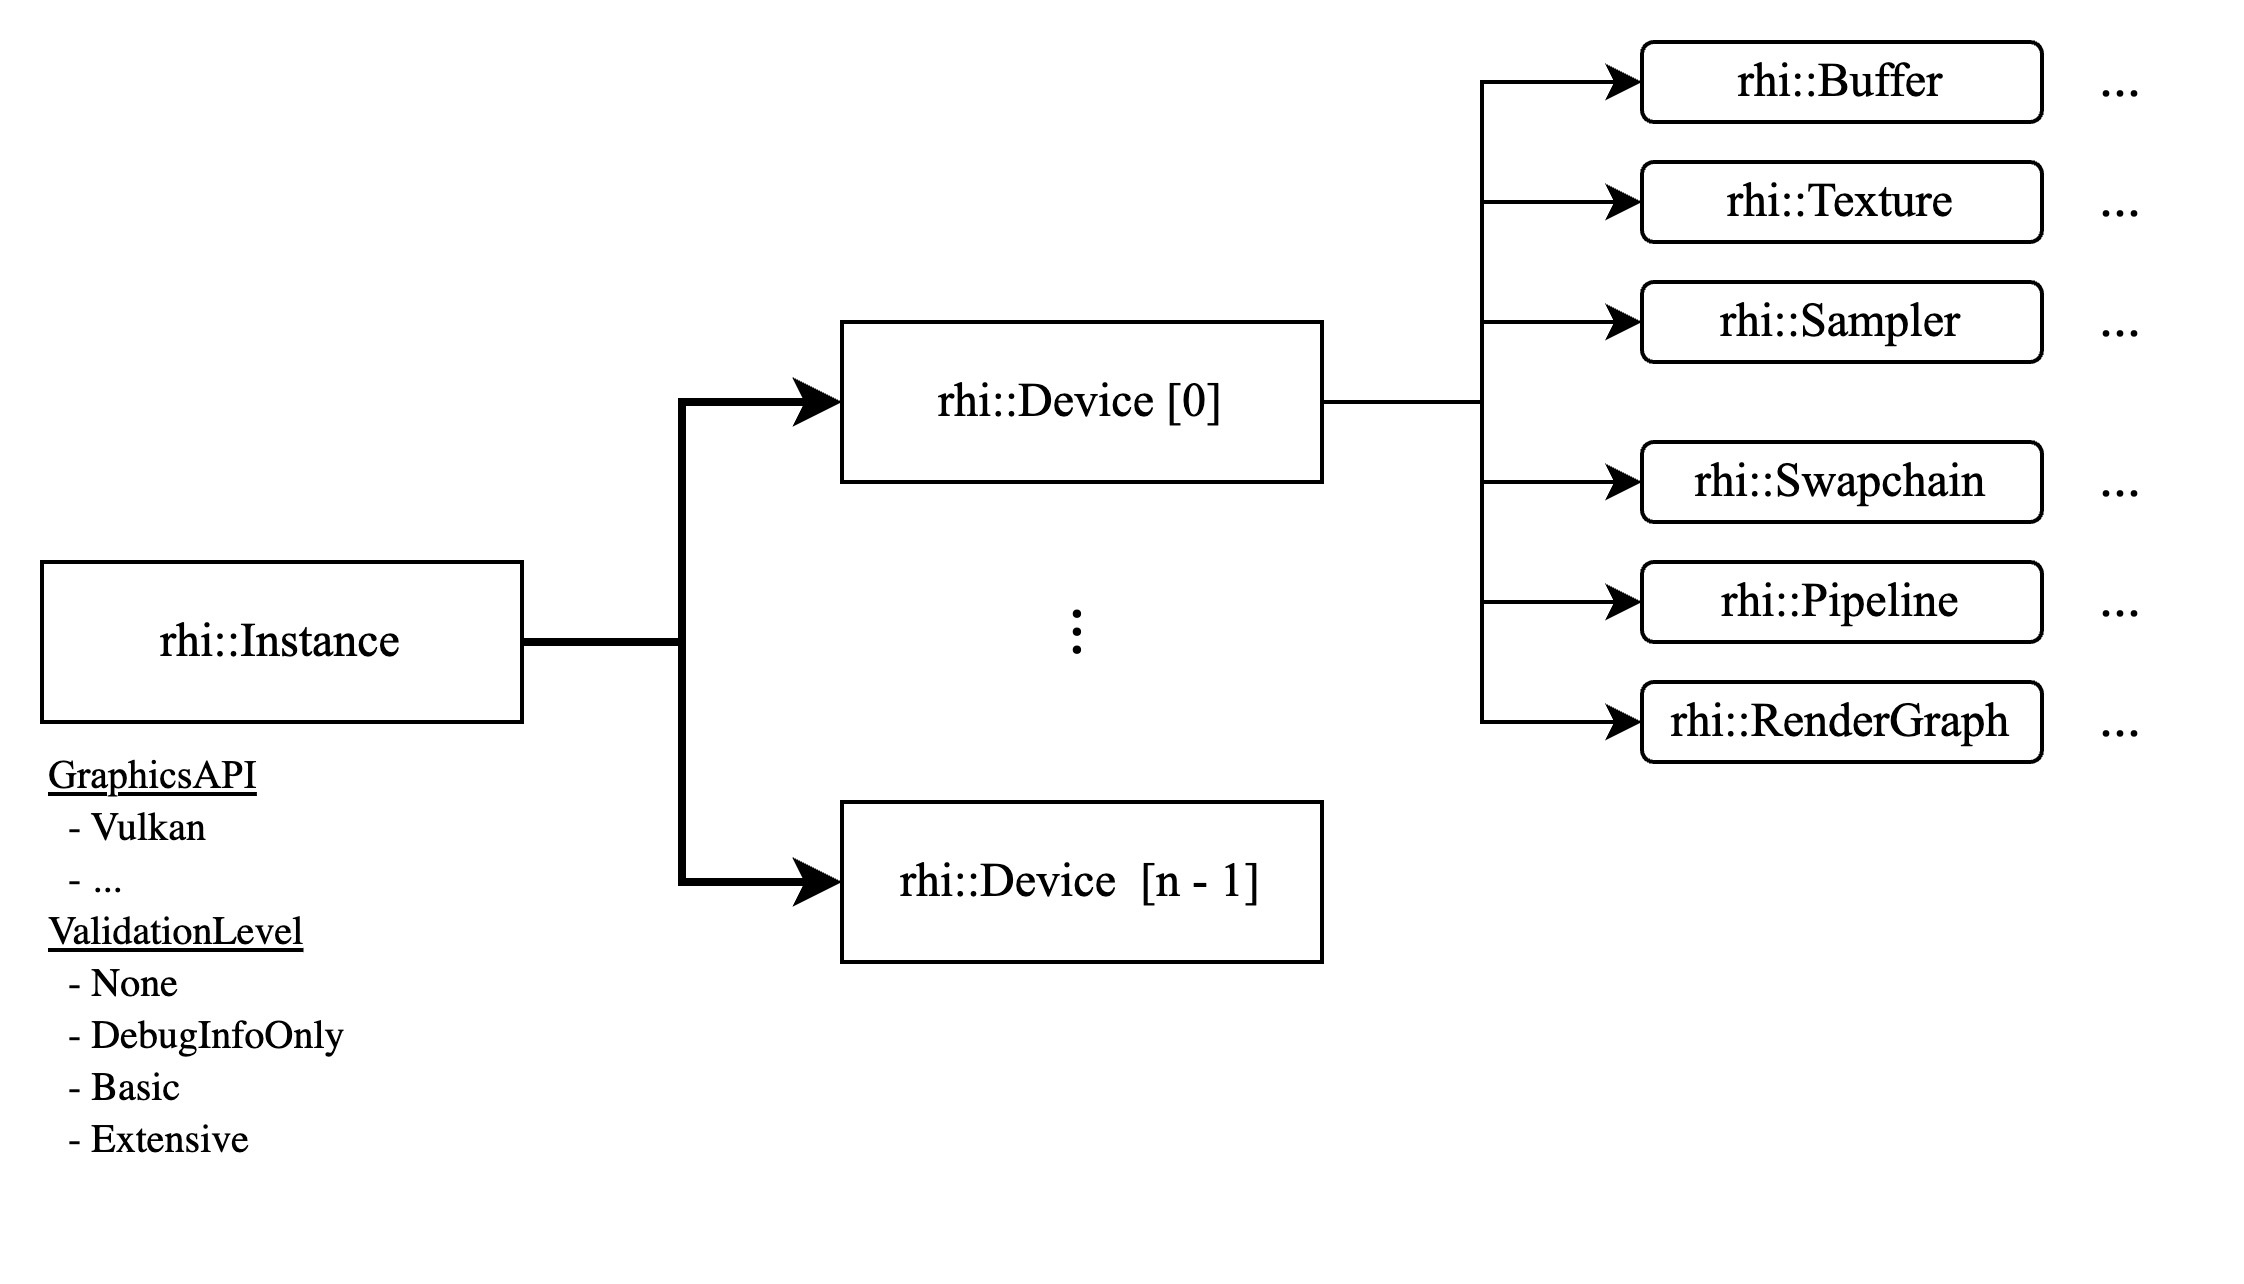
\includegraphics[scale=0.17]{rhi/rhi_classes.jpeg}
    \caption{Основные классы, представленные в RHI.}
    \label{fig:rhi_classes}
\end{figure}

\subsubsection{Device}
Как уже было сказано, современные графические API предоставляют объектный интерфейс. Поэтому конкретный графический процессор (далее \textit{device}) так же

\subsubsection{Ресурсы}
Работу 

\subsubsection{Рендер граф}
Рендер граф является одним из способов организации работы на GPU и представляет из себя ориентированный ациклический граф, где вершины являются вычислительными задачами, а ребра между ними задают зависимости в порядке исполнения этих задач. Концептуально работу с рендер графом можно разбить на три этапа - \textit{декларация}, \textit{компиляция} и \textit{исполнение}. На этапе декларации графа задаются вершины, а также ресурсы, которые будут использоваться. Вершина графа может быть одного из трех типов -- \textit{graphics}, \textit{compute} или же \textit{transfer}. Ресурсы, в свою очередь, могут быть либо вспомогательными, либо импортированными. Первыми владеет и управляет рендер граф, вторыми же он только пользуется. Каждому использованию ресурса присваивается некоторое уникальное целое число -- \textit{версия}. Пример декларации графической вершины представлен в листинге \ref{lst:render_graph_declaration}. Компиляцией занимается конкретная имплементация RHI, на этом этапе создаются все необходимые объекты для исполнения рендер графа. На этапе исполнения конкретная имплементация проходит в нужном порядке по вершинам, вызывает задачу, ассоциированную с данной вершиной на этапе декларации и занимается автоматически расстановкой синхронизации, контекста, отправляет работу на девайс и т.д.

\begin{minipage}[h]{0.95\textwidth}
\centering
\begin{cpp}[language=C++, caption={Пример декларации графической вершины рендер графа.}, label={lst:render_graph_declaration}]
auto rg_color = builder.DeclareImportTexture(...);
auto rg_depth = builder.DeclareTransientTexture(...);

builder.BeginRenderPass("Forward Pass");
builder.AddColorTarget(rg_color, ...);
builder.SetDepthStencil(rg_depth, ...);
builder.SetJob([](CommandBuffer& cmds) {
    ...
});
builder.EndRenderPass();
\end{cpp}
\end{minipage}

Одна из ключевых идей в моем RHI -- не предоставлять доступ к созданию и отправке на девайс командных буферов. Это заставляет выражать всю вычислительную работу с GPU посредством рендер графов. Данный подход позволяет более точечно оптимизировать каждую реализацию RHI с учетом особенностей конкретного графического API и аппаратного обеспечения, вместо того, чтобы пытаться обобщить работу с командными буферами между API.

Часто бывает необходимо декларировать временные ресурсы, чьи параметры зависят от других ресурсов. Например, это может быть буфер глубины, ведь его размер должен совпадать с размерами окна, т.е. главного рендер таргета. В связи с этим функции декларации временных ресурсов принимают структуру, похожую на обычную спецификацию ресурса, но у которой некоторые поля (такие как напр. размер) могут помимо точного значения принимать версию ресурса рендер графа, показывая зависимость. Пример такой декларации показан в \ref{lst:render_graph_dependent_texture_info}.

\begin{minipage}[h]{0.95\textwidth}
\centering
\begin{cpp}[language=C++, caption={Пример декларации зависимых временных ресурсов.}, label={lst:render_graph_dependent_texture_info}]
auto rg_color = builder.DeclareImportTexture(...);

rhi::RenderGraph::DependentTextureInfo depth_info{};
depth_info.extent.SetDependency(rg_color);
depth_info.format = rhi::Format::D32_SFLOAT;
depth_info.type   = rhi::TextureType::Texture2D;
depth_info.usage  = rhi::DeviceResourceState::DepthStencilTarget;
...
depth_info.name   = "Depth buffer";

auto rg_depth = builder.DeclareTransientTexture(depth_info);
\end{cpp}
\end{minipage}

\subsubsection{Рендер граф -- компиляция и реализация под Vulkan}

\begin{wrapfigure}{R}{0.305\textwidth}
    \centering
    \includegraphics[scale=0.12]{rhi/render_graph/topological_sort_graph.jpeg} 
    \caption{Граф зависимостей.}
    \label{fig:render_graph_topological_sort_graph}
\end{wrapfigure}

Первая часть компиляции рендер графа (топологическая сортировка) является универсальной для всех имплементаций. Предположим у нас есть $V$ вершин графа и уже расставленные ребра между ними, где ребро $(u, v)$, означает что вершина $v$ должна исполняться после $u$. В дальнейшем нам также понадобится глубина (или по-другому \textit{dependency level}) каждой вершины, обозначим ее $d(u)$. Она определяется как минимальная из всех возможных реберная длина пути от некоторой вершины $s$, в которую не ведут никакие ребра. За один обход в глубину графа мы сможем получить как глубины всех вершин, так и некоторую топологическую сортировку. Однако произвольная топологическая сортировка нам не подойдет. Необходимо, чтобы в получившейся сортировке глубины вершин монотонно не убывали. Для этого необходима дополнительная сортировка массива. Результат данной части алгоритма для графа \ref{fig:render_graph_topological_sort_graph} проиллюстрирован на диаграмме \ref{fig:render_graph_topological_sort_arrays}.

\begin{figure}[h]
    \centering
    \includegraphics[scale=0.15]{rhi/render_graph/topological_sort_array.jpeg}
    \caption{Первый массив -- произвольная топологическая сортировка, второй -- перестановка первого, упорядочивающая глубину по неубыванию (оставаясь при этом топологической сортировкой).}
    \label{fig:render_graph_topological_sort_arrays}
\end{figure}

% \begin{figure}
% \begin{minipage}{0.34\textwidth}
%     \centering
%     \includegraphics[scale=0.12]{render_graph/topological_sort_graph.jpeg}
%     \caption{Граф зависимостей. Переменной \textit{d} напротив каждой вершины обозначена глубина данной вершины.}
%     \label{fig:render_graph_topological_sort_graph}
% \end{minipage}
% \hfill
% \begin{minipage}{0.62\textwidth}
%     \centering
%     \includegraphics[scale=0.12]{render_graph/topological_sort_array.jpeg}
%     \caption{Первый массив -- произвольная топологическая сортировка, второй же является перестановкой первого, упорядочив по возрастанию глубину (оставаясь при этом топологической сортировкой).}
%     \label{fig:render_graph_topological_sort_arrays}
% \end{minipage}
% \end{figure}

Теперь избавимся от ненужных ребер графа для дальнейшего определения точек синхронизации командных очередей. Данная часть алгоритма основана на статье \cite{organizing_gpu_work_with_directed_acyclic_graphs} и идентична для всех современных графических API. Предположим, у нас есть $Q$ командных очередей. Также для каждой вершины нам известен индекс очереди, на которой она будет исполняться -- $queue\_idx(u) \in \{0,...,Q-1\}$. Прежде всего необходимо переиндексировать вершины так, чтобы внутри каждой очереди вершины шли по возрастанию, и для любой пары очередей $q_1, q_2 \in \{0,...,Q-1\}$, таких что $q_1 < q_2$, все вершины очереди $q_1$ имели индексы меньше, чем индексы всех вершин очереди $q_2$. Положим в качестве такой переиндекцации $\sigma(u) = sort\_idx(u) + queue\_idx(u) \cdot V + 1$. Также для каждой вершины введем так называемый \textit{Sufficient Synchronization Index Set} (сокращенно \textit{SSIS}), для каждой очереди показывающий индекс $\sigma$ вершины, с которой достаточно синхронизировать данную вершину. Формальное определение \textit{SSIS} представлено в равенстве \ref{eq:ssis_definition}. Граф с посчитанными \textit{SSIS} можно увидеть на диаграмме \ref{fig:cross_queue_graph_original}.

\begin{align}
    i_{q}(u) &= \left\{ \begin{array}{rcl}
        \sigma(u) & \mbox{если} & q = queue\_idx(u) \\
        0 & \mbox{иначе, если} & \forall v: (u, v) \notin E(G^R) \\
        \underset{d(v) \leq d(u)}{\underset{(u,v) \in E(G^R)}{\arg\max}} \{\sigma(v)\} & \mbox{иначе}
    \end{array}\right.&\\
    SSIS(u) &= \left( i_0(u), ..., i_{Q-1}(u) \right) \label{eq:ssis_definition}
\end{align}

\begin{figure}
    \centering
    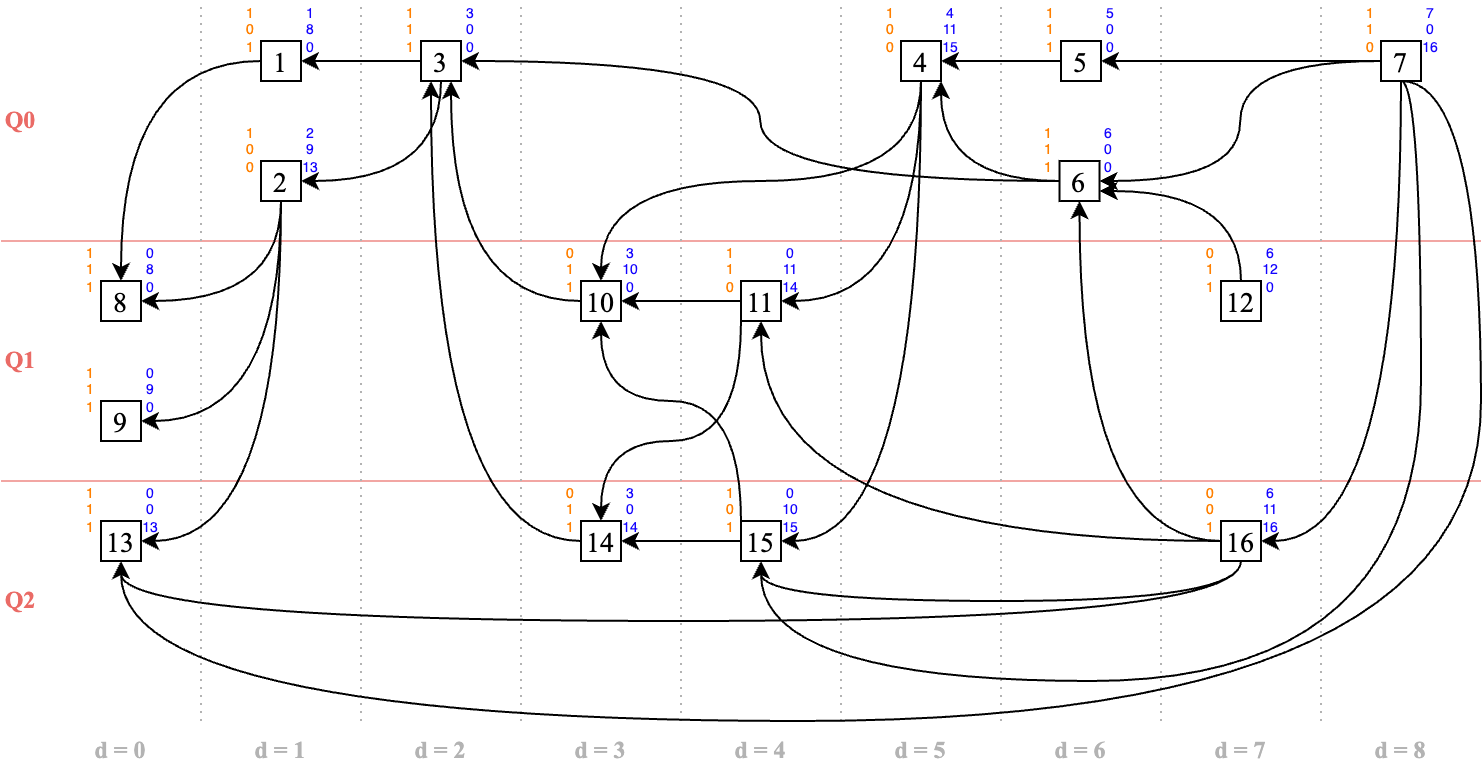
\includegraphics[scale=0.14]{rhi/render_graph/cross_queue_graph_original.jpeg}
    \caption{Изначальный реверс граф, где у каждой вершины справа синим светом подписан $SSIS$, слева оранжевым $final\_cover$, а индексация вершин показывает $\sigma(u)$.}
    \label{fig:cross_queue_graph_original}
\end{figure}

Строить новый граф без лишних ребер (назовем его $G^*$) будем итеративно. Для начала для каждой вершины посчитаем бинарный кортеж $cover$ из $Q$ элементов, каждый элемент которого показывает синхронизирована ли данная вершина с данной очередью. Дальше будем в цикле пытаться улучшить ситуацию, пока для всех вершин $cover$ не станет полностью из единиц. На каждой итерации раскрываются все вершины $u$, чьи $cover$ имеют нули. Раскрытие вершины $u$ происходит следующим образом: рассматриваются все вершины $v$, в которые идут ребра реверс графа из $u$, считается промежуточный $cover$ между только этими двумя вершинами, и если данное ребро улучшает глобальный $final\_cover(u)$, то мы запоминаем вершину $v$. Выбрав из всех таких $v$ наилучшую (по количеству единиц, которое она добавляет в $final\_cover(u)$), мы обновляем $final\_cover(u)$ и добавляем в граф $G^*$ ребро $(u, v)$. Полный алгоритм представлен в листинге \ref{lst:render_graph_cross_queue_graph}, а также первая итерация алгоритма проиллюстрирована на диаграмме \ref{fig:cross_queue_graph_first_iteration}.

\begin{minipage}[t]{0.95\textwidth}
    \centering
    \begin{pseudocode}[mathescape=true, caption={Построение графа $G^*$ с достаточным минимальным набором ребер для межочередной синхронизации}, label={lst:render_graph_cross_queue_graph}]

    function CoverScore($cover$):
        return $\sum_{q=0}^{Q-1} cover_q$

    $\forall u: final\_cover(u) \leftarrow (1, ..., 1)$
    $\forall u \forall q \in\{0, ..., Q-1\}: (\exists v: (u, v) \in E(G^R)) \implies final\_cover_q(u) \leftarrow 0$

    $covered\_all$ $\leftarrow$ false
    while not $covered\_all$:
        $covered\_all$ $\leftarrow$ true
        for $u \in G^R$:
            $v^* \leftarrow \emptyset$
            $cover^* \leftarrow final\_cover(u)$
            for $v \in G^R, (u, v) \in E(G^R)$:
                $cover \leftarrow (..., SSIS_q(u) \leq SSIS_q(v), ...)$
                if CoverScore($cover$) $>$ CoverScore($cover^*$):
                    $v^* \leftarrow v$
                    $cover^* \leftarrow cover$
                else if CoverScore($cover$) $=$ CoverScore($cover^*$) and $\sigma(v) > \sigma(v^*)$
                    $v^* \leftarrow v$
                    $cover^* \leftarrow cover$
            if $v^* \neq \emptyset$:
                $final\_cover(u) \leftarrow final\_cover(u) | cover^*$
                $G^* \leftarrow G^* \cup (u, v^*)$
            if CoverScore($final\_cover(u)$) $\neq Q$:
                $covered\_all$ $\leftarrow$ false
    \end{pseudocode}
\end{minipage}

\begin{figure}
    \centering
    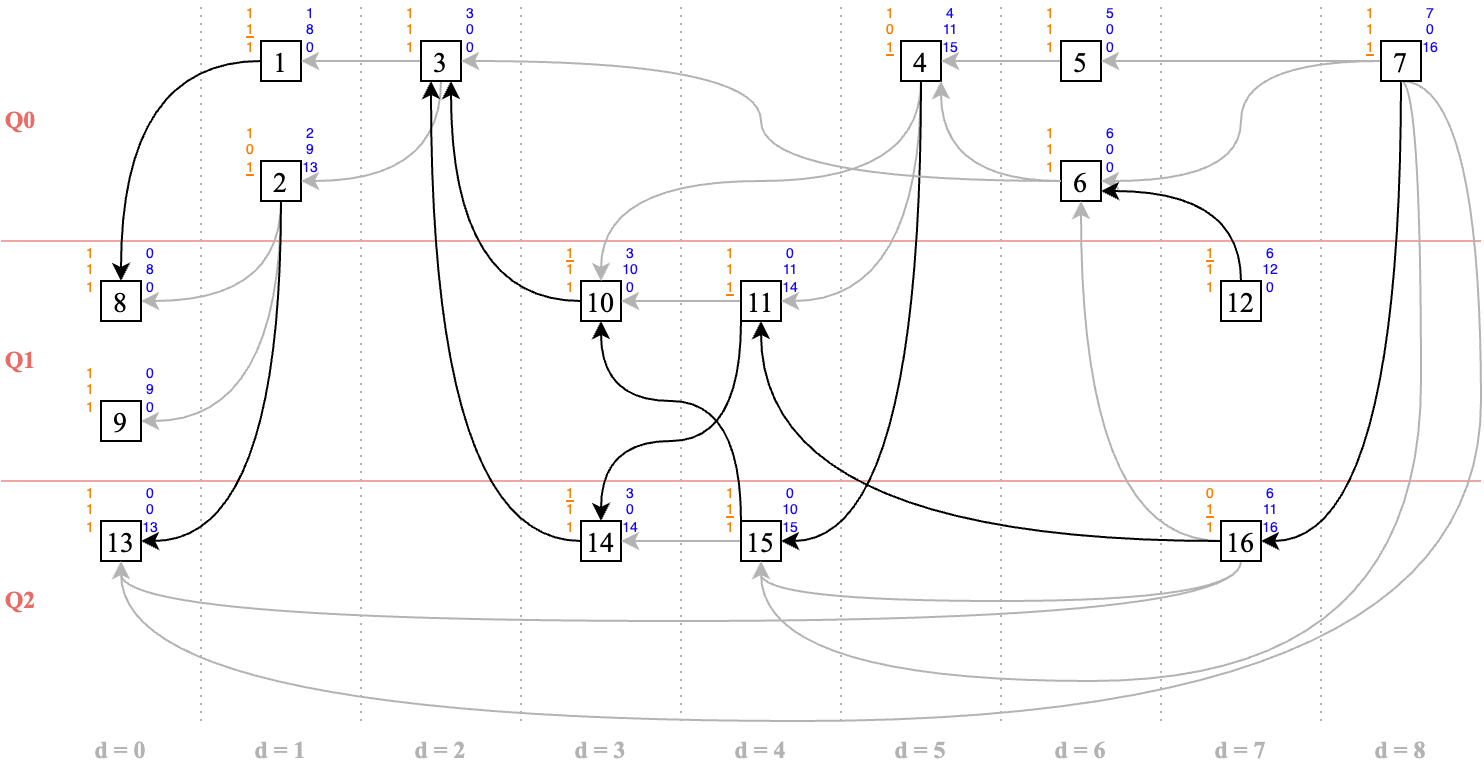
\includegraphics[scale=0.14]{rhi/render_graph/cross_queue_graph_first_iteration.jpeg}
    \caption{Первая итерация алгоритма построения $G^*$.}
    \label{fig:cross_queue_graph_first_iteration}
\end{figure}

Дальше идет часть компиляции, уникальная для Vulkan. Нам необходимо расставить сабмиты, а также синхронизацию между ними при помощи семафоров, примитивов синхронизации командных очередей. В новых версиях Vulkan появились так называемые временные семафоры, способные хранить 64-битное число вместо бинарного флага. Именно их и предлагается использовать. Сабмиты ставятся в конце каждой очереди, а также после каждого слоя глубины, на котором есть вершины, в которые идут ребра графа $G^*$. На каждую очередь выделено по одному временному семафору. Поскольку значения должны монотонно расти, каждое значение можно представить как $Timepoint(frame\_idx, submit\_idx) = frame\_idx \cdot V + submit\_idx$. В данном определении $V$ -- произвольное число, заведомо большее числа сабмитов на каждой очереди, а $submit\_idx$ -- индекс сабмита на конкретной очереди в 1-индексации. Дальше достаточно на основе ребер $G^*$ расставить значения ожидания/сигнала на каждом сабмите. Финальную версию графа $G^*$ с выставленными сабмитами можно увидеть на диаграмме \ref{fig:cross_queue_graph_submits}.

Немаловажной частью работы с Vulkan также является ручная расстановка барьеров исполнения для ресурсов. Если ресурс используется исключительно в одной очереди, то автоматическая расстановка барьеров в таком случае тривиальна, хотя и требует внимательного рассмотрения всех параметров. Сложность возникает, когда ресурс используется на нескольких очередях. Самый простой вариант решения данной проблемы -- это создание всех ресурсов с указанием автоматического кросс-очередного использования. Этот подход может повлиять на производительность, например, делая невозможным использование \textit{delta color compression} \cite{optimising_a_aaa_vulkan_title_on_desktop}. Второй же подход -- расставлять барьеры с \textit{queue ownership transfer}. В целом, в текущей имплементации рендер графа расстановка данных барьеров не требует больших усилий, поэтому этот подход более предпочтительный.

\begin{figure}
    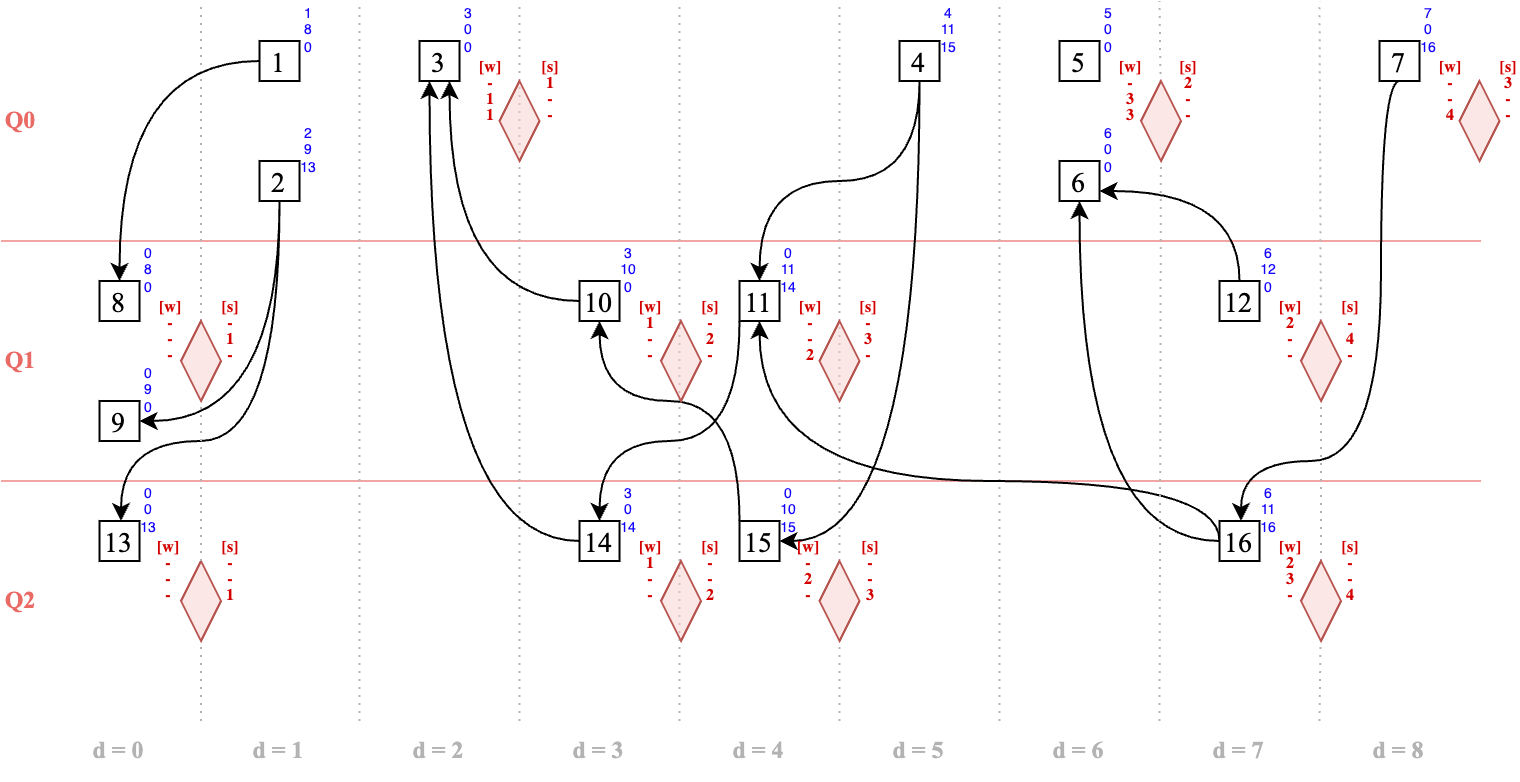
\includegraphics[scale=0.155]{rhi/render_graph/cross_queue_graph_submits.jpeg}
    \caption{Финальный граф $G^*$ с выставленными сабмитами. Слева от каждого сабмита подписаны значения для ожидания на каждую очередь, а справа -- значения для сигнала.}
    \label{fig:cross_queue_graph_submits}
\end{figure}

\subsubsection{Структура кадра}

\subsection{Asset management}
\subsubsection{Регистр ресурсов}
\subsubsection{Импорт внешнего контента}
\subsubsection{Загрузка и время жизни ресурсов}

\subsection{ECS}
\subsubsection{Объекты и компоненты}
\subsubsection{Граф исполнения систем}
\subsubsection{Идеи по использованию внешними модулями}

\subsection{Shader system}
\subsubsection{Формат}
\subsubsection{Стек деклараций}
\subsubsection{Кодогенерация}
\subsubsection{Высокоуровневый шейдер}

\subsection{Рендерер}
В данной главе представлена имплементация высокоуровнего рендерера в целях тестирования дизайна и реализации RHI. Современный высокоуровневый рендерер должен быть модульным, удобным в использовании, а также в идеальном случае быть полностью конфигурируемым, включая возможность написания кастомного решения специально под нужды конкретного игрового проекта. Дизайн, представленный в данной работе (см. рисунок \ref{fig:renderer_design}) стремится решить все эти проблемы. Рендерер состоит из абстрактных компонент -- IRenderFeature. Каждая из них декларирует вершины рендер графа, а также ECS системы (в основном предназначенные для агрегирования данных из компонент сущностей на сцене). Коммуникация между различными IRenderFeature сделана через абстрактный Context, способный содержать произвольные данные.

\begin{figure}
    \centering
    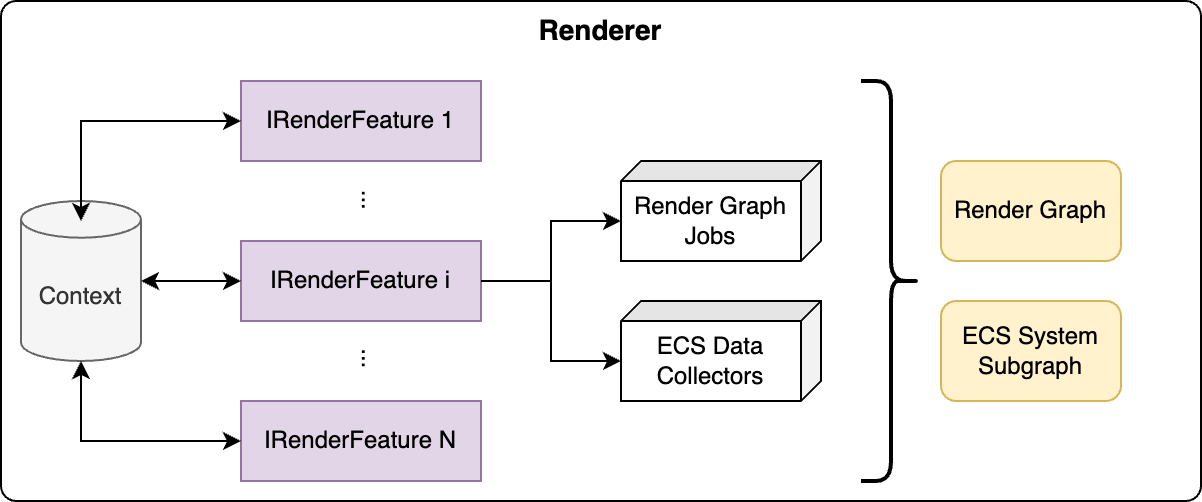
\includegraphics[scale=0.5]{renderer/renderer.png}
    \caption{Дизайн рендерера}
    \label{fig:renderer_design}
\end{figure}

Конкретные имплементации IRenderFeature можно классифицировать на: отрисовку геометрии, отрисовку процедурных объектов, а также эффекты постобработки. Поэтому в качестве рендерера по-умолчанию были реализованы методы рендеринга из всех данных классов в качестве проверки дизайна.

\subsubsection{Отрисовка геометрии}


\subsubsection{Симуляция и отрисовка частиц}
\subsubsection{Эффекты постобработки}
